\documentclass[12pt,a4paper]{article}	%only 10 to 12 working in article
\usepackage[left=2cm, right=2cm, top=1cm]{geometry}

\usepackage{graphicx}
\usepackage{subcaption}
%packages for inserting image

\usepackage{upgreek}
%type greek letter command between $' '$ !!

\title{1.Torsion Test : Theory and Experimental Procedure}
\date{\vspace{-5ex}}	%to skip printing the dat in the title
\begin{document}
\maketitle
\section{Theory of Pure Torsion}
The Torsion Test is based on the \textbf{Theory of Pure Torsion}\\

If a material is subjected to twisting by the application of a couple a shear stress will be induced within the material. If a couple is applied to a cylindrical rod in such a way that the axis of the couple is coincident with the axis of the rod, then the rod is said to be subject to pure torsion. At any point within the cross-section of a rod subjected to pure torsion, there will be a pure shear stress established in a direction normal to the radius of the rod at that point.\\
	\begin{figure}[h!]
	\centering
	\begin{subfigure}[b]{0.5\linewidth}
		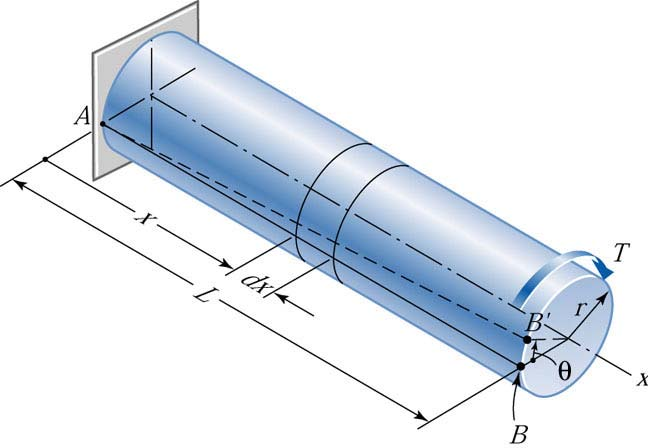
\includegraphics[width=\linewidth]{Ok.png}
		\caption{Circular beam subjected to torque T}
	\end{subfigure} \hspace{10mm}%to add space 
	\begin{subfigure}[b]{0.4\linewidth}
		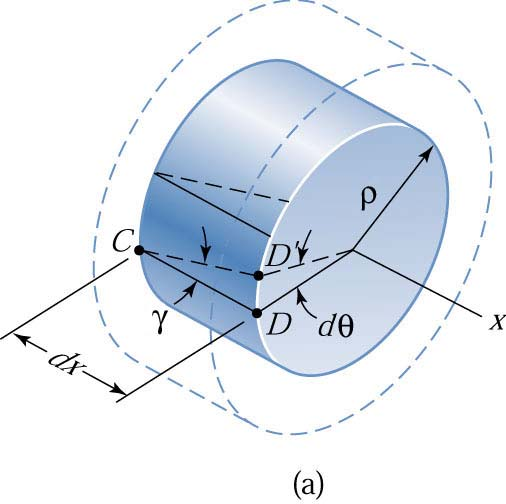
\includegraphics[width=\linewidth]{Ok1.png}
		\caption{dx section}
	\end{subfigure}
\end{figure}
\\
The assumptions made in the Theory of Pure Torsion or made in deriving the equation for pure torsion are as follows:
\thispagestyle{empty}	%To supress the printing of page number
\begin{itemize}
\item The material is homogeneous and isotropic
\item Hooke's law is obeyed by the material.i.e deformation are withing within proportionality limit \textbf{(Important)}
\item The shaft is circular in section and remains planar even after torque is applied on it
\item The cross-section of the shaft remains uniform throughout.
\item The shaft is subjected to pure torque only.
\item The shaft is not subjected to any initial torque. i.e initial deflection is zero
\item The stress of the material should not exceed the elastic limit i.e no permanent deformation is caused due to loading
\end{itemize}

\pagebreak
The torsion equation is given as follows:
\[\frac{T}{J} = \frac{\tau}{r} = \frac{G \theta}{L}\]
The given equation hold for the condition of \textbf{Pure Torque}.Every diameter of the material rotates through the same angle i.e The shear strain $\gamma$ varies linearly in the radial direction
\bigbreak
\thispagestyle{empty}	%To supress the printing of page number
\begin{figure}[h!]
	\centering
	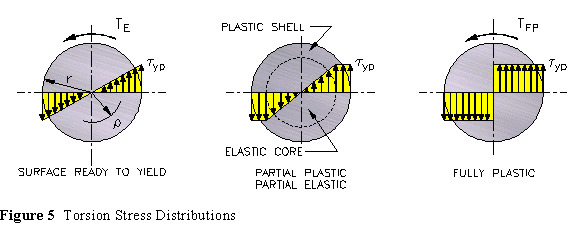
\includegraphics[width=\linewidth]{Pure_Torque.jpg}
	\caption{Types of Torques acting on a cross section:(a)Pure Torsion, (b) Partially Elastic Torsion, (c) Fully Plastic Torsion}
\end{figure}
\bigbreak
Thus, continuing with the Pure Torsion Assumption,we find the Shear Modulus (G) through our experiment.

\section{Procedure}
\begin{enumerate}
\item Measure the length and diameter of the Aluminium 6061 Rod
\item Subtract the Zero Errors to obtain the true dimensions
\item Weigh the masses to be used for the experiment
\item Clamp the rod in the Torsion Test Apparatus
\item Check for any zero error present in the apparatus. If possible,set the reading to zero when no mass is attached
\item Gradually add weights and note down the reading of the deflection while loading
\item After having put all the weights,remove them one by one and note down the reading in deflection while unloading as well
\item Complete 20 such cycles of loading and unloading
\item For each reading calculate Shear Stress and Shear Strain using the formula:

\[Shear Stress = \frac{Torque*Radial Distance}{J}=\frac{(mgd)*r}{J}\]\\
and
\[Shear Strain = \frac{Deflection(radian)*Radial Distance}{L} = \frac{\theta r}{L}\]\\
where,\\
m = mass attached to the apparatus\\
Radial Distance = from centroidal longitudinal axis to the outer surface\\
d = length of lever used to apply torque in Torsion Test Apparatus
\item Plot the Data points for each cycle
\item Sketch the best fit straight line through the points for each plot
\item Measure the Slope of the best fit line\\

Slope of the best fit line in a Stress vs Strain Plot gives the value of the Young's Modulus\\

Since we made a plot between Shear Stress and Shear Strain, the Slope of the best fit line gives us the value of the Shear Modulus (G)
\end{enumerate}
\thispagestyle{empty}	%To supress the printing of page number

\end{document}